\section{Laboratorium I}\label{sec:lab-1}

\subsection{Wybrany sprzęt}\label{subsec:lab1-hw}

Oficjalny moduł Fundacji Raspberry Pi -- \emph{Sense HAT} -- zawiera żyroskop, akcelerometr, magnetometr, barometr,
termometr, higrometr, czujnik oświetlenia, joystick, oraz~matrycę $8\,\times\,8$ pikseli RGB\thinspace\cite{sensedoc}.

Część dostępnej funkcjonalności pokrywa~się z~pozostałymi dostępnymi modułami, w~związku z~czym do~tego~laboratorium
wykorzystana~została funkcjonalność \emph{Inertial Measurement Unit} -- żyroskop, akcelerometr, magnetometr, a~także
matryca pikseli w~celu symulacji działania kompasu.

Z~powodu dużych zakłóceń magnetycznych spowodowanych obecnością metalowych elementów w~większości pomieszczeń uczelni,
utworzony kompas nie~będzie bardzo dokładny, jednak dostatecznie pokazuje działanie podobnych urządzeń np.\
w~telefonach czy~technologiach \emph{Full Body Tracking} popularyzowanych w~kręgach fanów wirtualnej rzeczywistości.
Rozwiązania~te poza~zdecydowanie bardziej wyspecjalizowanym doborze elementów sprzętowych i~bardziej zaawansowanym
oprogramowaniu kompensującym wpływ czynników zewnętrznych opierają~się fundamentalnie na~tej~samej zasadzie działania.

W~celu redukcji niedokładności instrukcja zawiera zadanie kalibracyjne, jego~wynik zależy jednak od~warunków środowiska
i~dokładności wykonania, więc~jest~jedynie krokiem referencyjnym pokazującym istnienie podobnego procesu po~stronie
producenta zintegrowanych urządzeń.

\subsection{Dodatkowe oprogramowanie}\label{subsec:lab1-sw}

W~tym laboratorium wykorzystana~jest oficjalna biblioteka \emph{sense\_hat}\thinspace\cite{senselib}.
Jest to zalecany i~najprostszy sposób wykorzystania możliwości sensorów modułu \emph{Sense HAT}, gdyż biblioteka
zapewnia wysokopoziomowe interfejsy do~obsługi zarówno czujników, jak~i~matrycy.
Dzięki temu wykorzystanie sprzętu jest~bliżej paradygmatowi deklaratywnemu, bez~potrzeby zrozumienia niskopoziomowych
detali komunikacji przeprowadzanej przez~urządzenia.

Zastosowanie tej~biblioteki stanowi łagodne wprowadzenie do~dalszych zadań realizowanych w~środowisku marimo.
Głównym jej~elementem jest~klasa \emph{SenseHat}, która zbiera zdefiniowane funkcje pod~jedną nazwą, pozwalając
środowisku marimo na~wyświetlanie podpowiedzi w interfejsie graficznym (rys.~\ref{fig:marimosuggestion}).

\begin{figure}[H]
  \centering
  \includegraphics[width=0.5\linewidth]{media/marimo_suggestions}
  \caption{Podpowiedzi w interfejsie graficznym marimo}
  \label{fig:marimosuggestion}
\end{figure}

\subsection{Rozwiązanie}\label{subsec:lab1-sol}

Rysunek~\ref{fig:sensehatlab} to~fragment instrukcji laboratoryjnej opisujący pierwsze z~zadań, jakim~jest
przeprowadzenie procesu kalibracji sensorów inercyjnych.
Pokazuje~on i~wyjaśnia kolejne kroki niezbędne do~wykonania podstawowego procesu kalibracji, co~znacząco zwiększa
dokładność późniejszych pomiarów oraz stabilność danych.
Instrukcja zwraca uwagę na prawidłowe ułożenie urządzenia w celu ograniczenia zakłóceń magnetycznych.

\begin{figure}[H]
  \centering
  \includegraphics[width=0.9\linewidth]{media/sense_hat_lab}
  \caption{Fragment instrukcji na temat \emph{Sense HAT}}
  \label{fig:sensehatlab}
\end{figure}

Na rysunku~\ref{fig:compass} zaprezentowany jest wynik uruchomienia rozwiązanego laboratorium.
Podobnie do~standardowego kompasu kierunki północy i~południa są~reprezentowane w~kolorach czerwonym i~białym.

\begin{figure}[H]
  \centering
  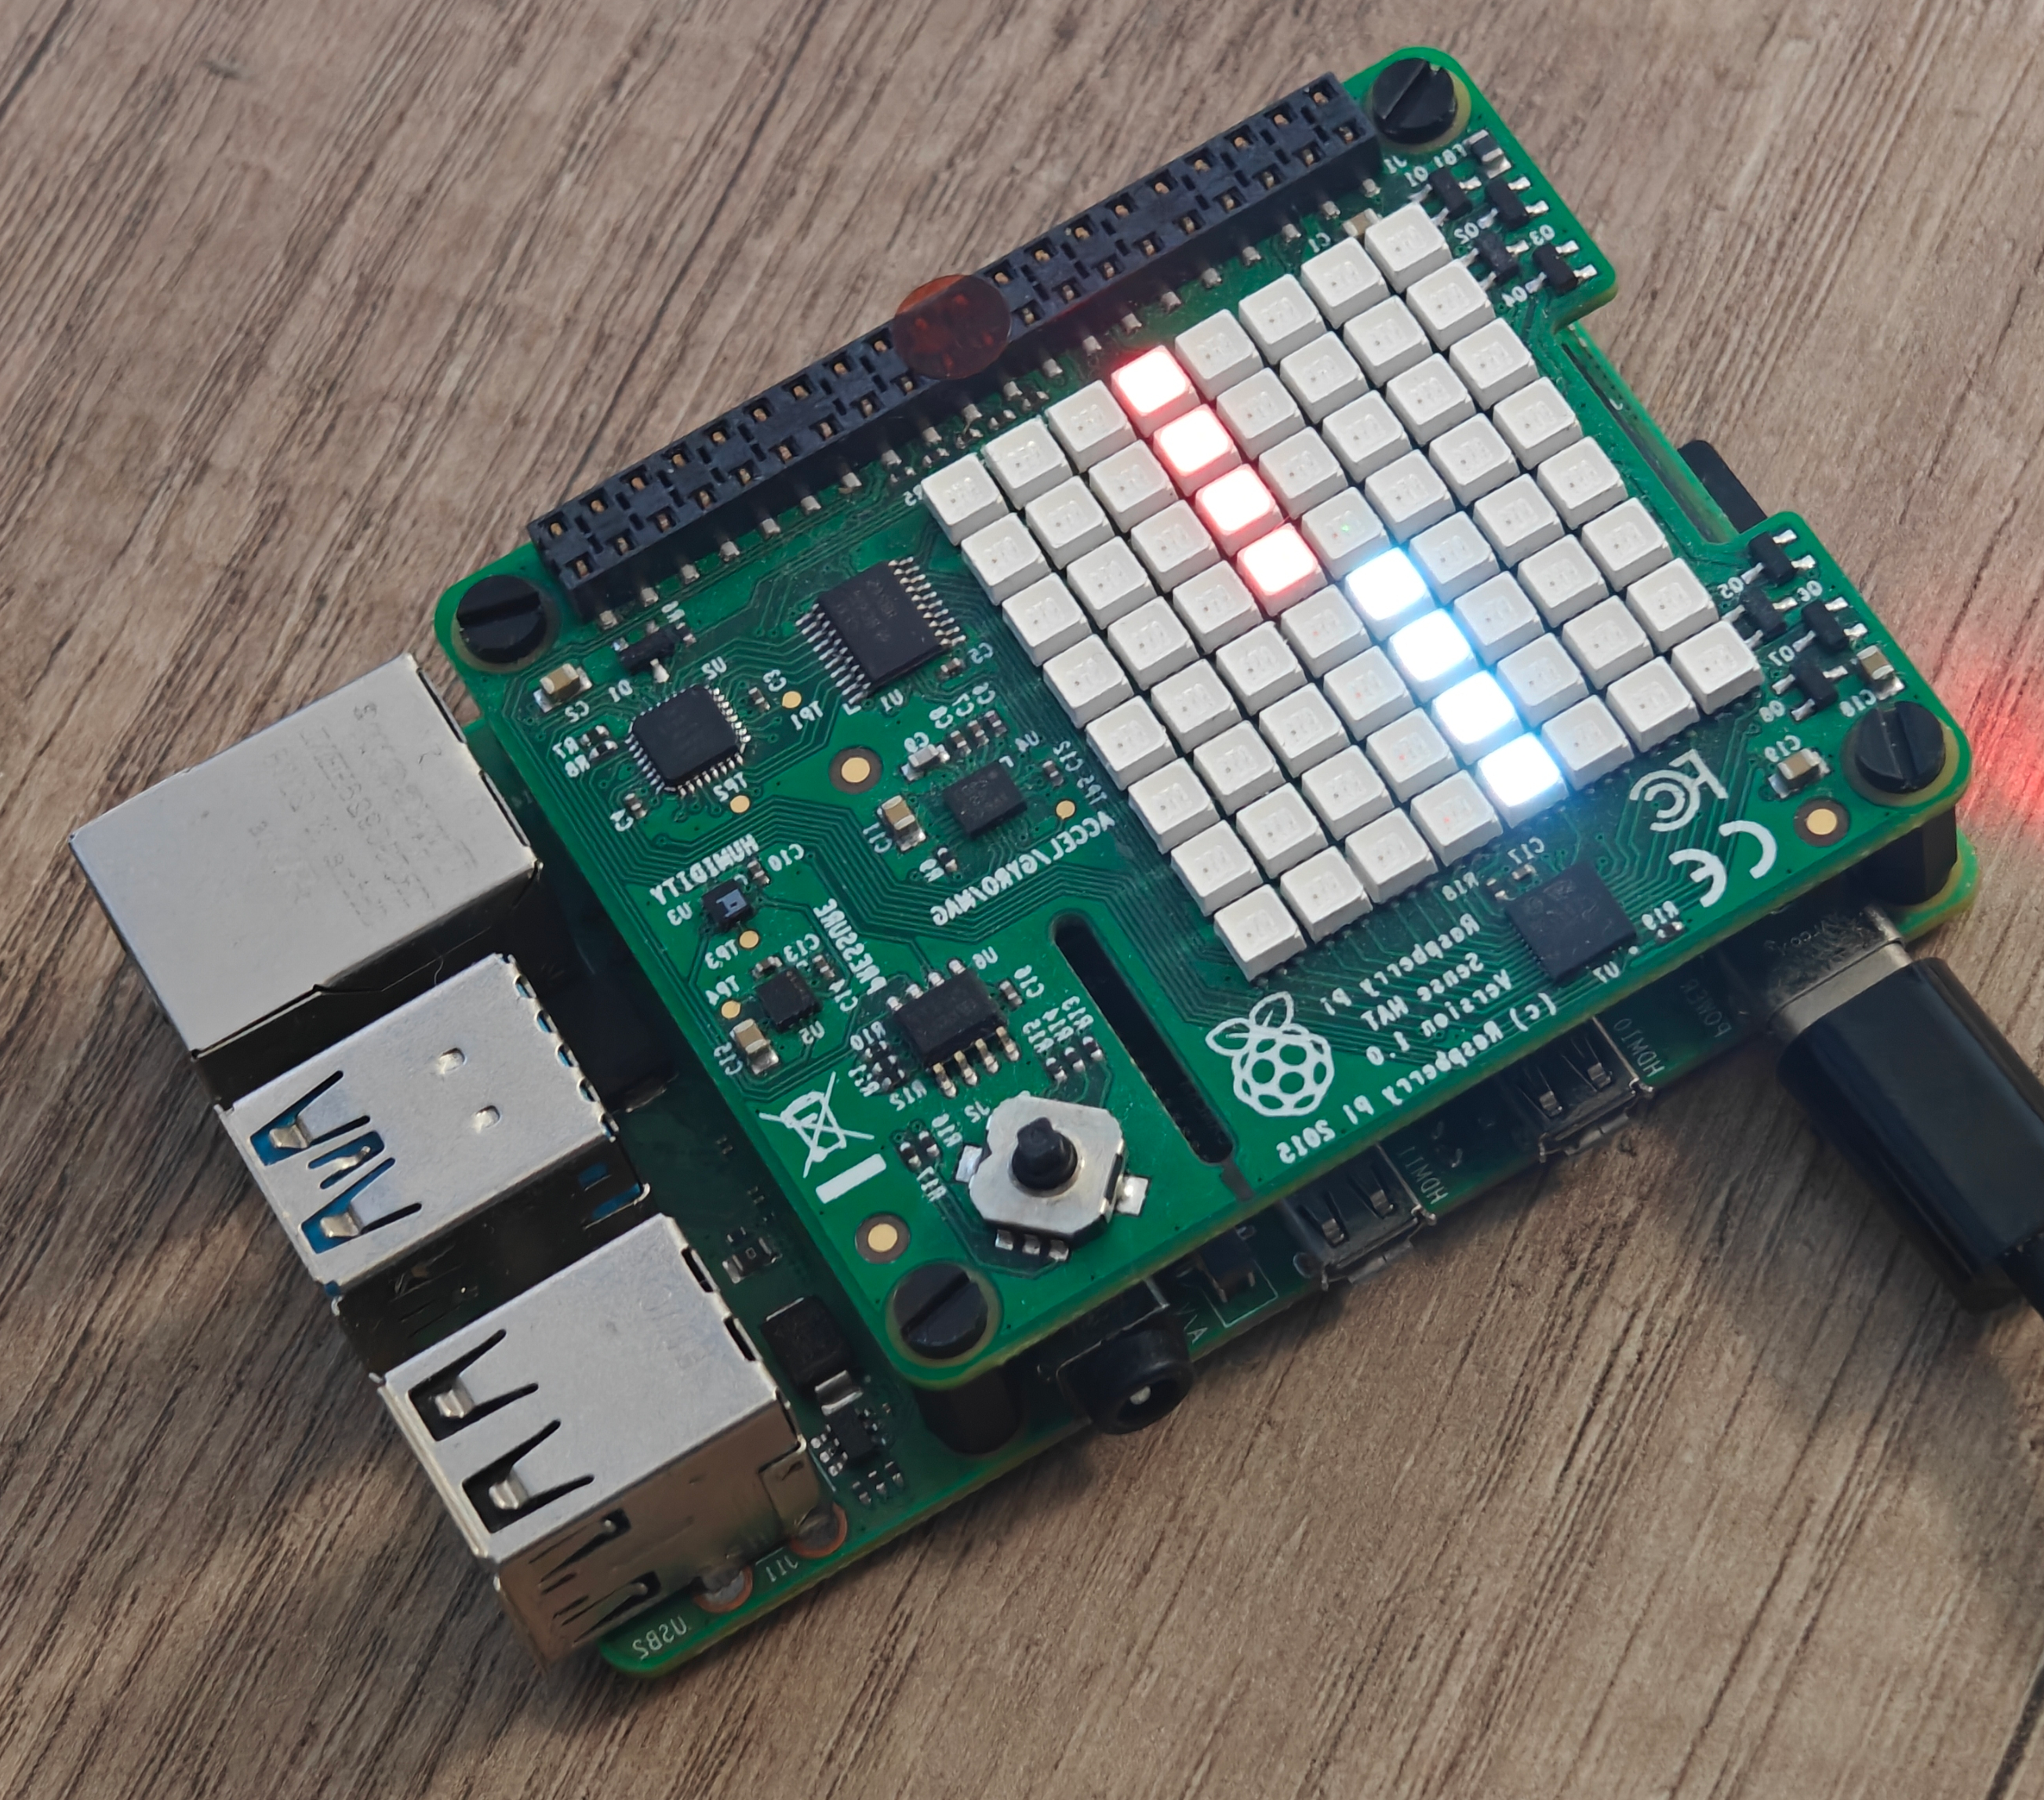
\includegraphics[width=0.6\linewidth]{media/compass}
  \caption{Uruchomiony program pierwszego laboratorium}
  \label{fig:compass}
\end{figure}
